\chapter{Improving CNN Performance Accuracies With Min–Max Objective}

{\small \textbf{Authors}\\
Weiwei Shi, Yihong Gong, \textit{Senior Member, IEEE}, Xiaoyu Tao, Jinjun Wang, \textit{Member, IEEE},
and Nanning Zheng, \textit{Fellow, IEEE}\\ \\
IEEE TRANSACTIONS ON NEURAL NETWORKS AND LEARNING SYSTEMS\\VOL. 29, NO. 7, JULY 2018}

\section{Proposed Method}

In this paper we are going to present a new method whose aim is to obtain better performance on CNNs without requiring any complication in terms of the structure of the network. The problem we want to focus on is the invariance of the features. More specifically, when a CNN is dealing with a problem of image classification or object detection, there might be the chance that even though we are trying to detect an object that we are supposed to recognize (because its image is among the training samples) we end up having problems. This eventuality might occur if the image given as input has been rotated, translated or something else. For this reason, the vector that represents the features of the desired object, changes and it is difficult to detect what we are looking for. That is why, through the proposed method of this paper, we aim at doing basically two operations.\\ \\
The first one is to compact the best we can each manifold that represents a single class. The second one is to increase as much as possible the distance between each manifold among different classes. By doing so, we can face way better changes involving viewing angles, position, light intensity etc. The method is called \textit{Min-Max Objective} and is applied to the layer closest to the output layer. Before of going any further it is important to say that it seems to be necessary to apply different operations on CNNs than the already well-known regularization ones. For instance, it has been proved that increasing the number of layers does not mean that performance is going to be better. As well as enlarging datasets by augmenting the training samples turns out to provide small improvements. For this reason, Min-Max Objective is proposed and it aims at minimizing the \textit{within-manifold}, and maximizing the \textit{between-manifold}. In order to be clearer, the within-manifold represents how compact a manifold is for a specific class, while the between-manifold is how far each manifold is from the others.\\ \\
As our goal is to minime the classification error, we end up with the following cost function

\begin{equation}
    \label{eq:04_1}
    \min\limits_{\mathcal{W}} L = \sum_{i=1}^n \ell(\textbf{X}_i,c_i;\mathcal{W})+\lambda\mathcal{L}(\mathcal{X}^{(k)},\textbf{c})
\end{equation}\\
where $\ell(\textbf{X}_i,c_i;\mathcal{W})$ is the classification error of the image $\textbf{X}_i$ and $\mathcal{L}(\mathcal{X}^{(k)},\textbf{c})$ is the proposed Min-Max objective. As the Min-Max objective is defined as

\begin{equation}
    \label{eq:04_2}
    \mathcal{L}(\mathcal{X}^{(k)},\textbf{c}) = \frac{S^{(B)}}{S^{(W)}}
\end{equation}\\
where $S^{(B)}$ is the between-manifold distance and $S^{(W)}$ the within-manifold distance, we come up with the final cost function that now is

\begin{equation}
    \label{eq:04_3}
    \min\limits_{\mathcal{W}} L = \sum_{i=1}^n \ell(\textbf{X}_i,c_i;\mathcal{W})-\lambda\frac{S^{(B)}}{S^{(W)}}
\end{equation}\\

\section{Experimental Results}

Experimental results have been evaluated on five datasets and on two applications. Datasets are CIFAR10 \citep{CIFAR10and100}, CIFAR100 \citep{CIFAR10and100}, MNIST \citep{MNIST}, SVHN \citep{SVHN}, ImageNet \citep{ImageNet12} and \citep{LFW}, while the applications are image classification and face verification. The results obtained show that if the Min-Max Objective is applied on the layer closest to the output layer we end up with better performance on the CNN. Moreover, in order to visualize the feature extracted and how well they were separated, t-SNE has been used. t-SNE is a tecnique used for dimensionality reduction and it is quite clear that by using the Min-Max Objective has been possible to obtain a more robust separability as shown in Figure \ref{eq:04_1}.\\

\begin{figure}[h!]
    \centering
    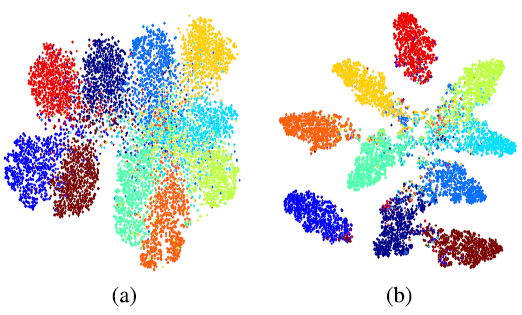
\includegraphics[scale=0.60]{images/04_1.png}
    \caption{Example of t-SNE visualization. (a) without t-SNE. (b) with t-SNE.}
    \label{fig:04_1}
\end{figure}

\FloatBarrier